\documentclass{article}
\usepackage{tikz}

\begin{document}

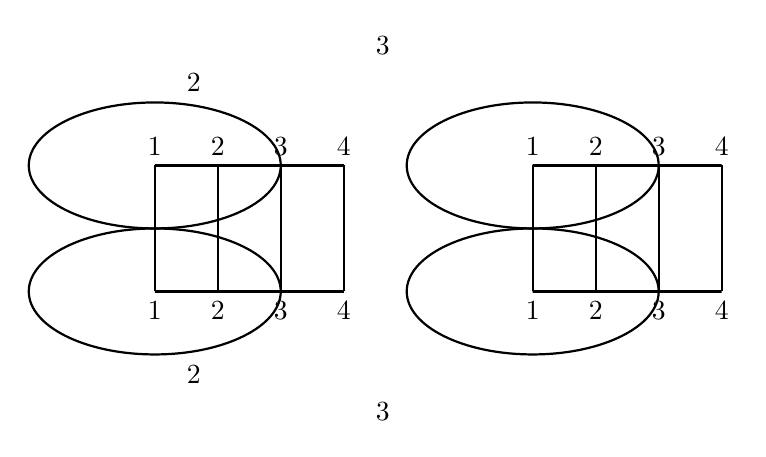
\begin{tikzpicture}[scale=0.8]
    % Define coordinates for nodes
    \foreach \x in {1,...,4} {
        \coordinate (a\x) at (\x, 0);
        \coordinate (b\x) at (\x, -2);
    }
    
    % Draw the first diagram
    \draw[thick] (a1) -- (a2) -- (a3) -- (a4) -- cycle;
    \draw[thick] (b1) -- (b2) -- (b3) -- (b4) -- cycle;
    \draw[thick] (a1) -- (b1);
    \draw[thick] (a2) -- (b2);
    \draw[thick] (a3) -- (b3);
    \draw[thick] (a4) -- (b4);
    
    % Label the nodes with numbers
    \foreach \x in {1,...,4} {
        \node at (a\x) [above] {\x};
        \node at (b\x) [below] {\x};
    }
    
    % Draw ellipses around the nodes
    \draw[thick] (a1) ellipse (2cm and 1cm);
    \draw[thick] (b1) ellipse (2cm and 1cm);
    
    % Add labels to the ellipses
    \node at (current bounding box.north) [above] {2};
    \node at (current bounding box.south) [below] {2};
    
    % Draw the second diagram
    \begin{scope}[xshift=6cm]
        \foreach \x in {1,...,4} {
            \coordinate (a\x) at (\x, 0);
            \coordinate (b\x) at (\x, -2);
        }
        
        \draw[thick] (a1) -- (a2) -- (a3) -- (a4) -- cycle;
        \draw[thick] (b1) -- (b2) -- (b3) -- (b4) -- cycle;
        \draw[thick] (a1) -- (b1);
        \draw[thick] (a2) -- (b2);
        \draw[thick] (a3) -- (b3);
        \draw[thick] (a4) -- (b4);
        
        % Label the nodes with numbers
        \foreach \x in {1,...,4} {
            \node at (a\x) [above] {\x};
            \node at (b\x) [below] {\x};
        }
        
        % Draw ellipses around the nodes
        \draw[thick] (a1) ellipse (2cm and 1cm);
        \draw[thick] (b1) ellipse (2cm and 1cm);
        
        % Add labels to the ellipses
        \node at (current bounding box.north) [above] {3};
        \node at (current bounding box.south) [below] {3};
    \end{scope}
\end{tikzpicture}

\end{document}